% Chapter 2

\chapter{State of the Art: Agentic AI and Small Language Models in Healthcare} % Main chapter title

\label{chap:Chapter2} % For referencing the chapter elsewhere, use \ref{chap:Chapter2}

%----------------------------------------------------------------------------------------

\section{Research Methodology}

The systematic literature review was conducted following the PRISMA 2020 statement \cite{page2021prisma}, a framework designed to ensure transparency and reproducibility in systematic reviews. This methodology was selected for several compelling reasons that align with the nature of this research domain. First, the fields of Agentic AI, Small Language Models, and Vision-Language Models are characterized by rapid innovation cycles, with foundational architectures and benchmark results being superseded within months of publication. PRISMA's structured approach ensures that the evidence synthesis captures this dynamism while maintaining methodological rigor. Second, the framework's emphasis on explicit documentation of search strategies, inclusion criteria, and study selection processes enhances the reproducibility of findings---a critical consideration given the interdisciplinary nature of this work spanning computer science, medical informatics, and clinical dermatology.

The review process was structured into four distinct phases: (1) identification of relevant studies through systematic database searching; (2) screening of titles and abstracts based on predefined inclusion criteria; (3) eligibility assessment of full-text articles against methodological quality standards; and (4) qualitative synthesis of the selected studies to address the defined research questions. The temporal scope of the search spanned publications from January 2023 to January 2026, a period deliberately chosen to capture the rapid maturation of Small Language Models following the release of instruction-tuned models such as Llama-2, Mistral, and Phi-2. Studies published before 2023 were excluded from the systematic review but referenced as foundational works where necessary to establish theoretical context.

Quality assessment of the selected studies followed a structured appraisal protocol designed specifically for this research domain. Each study was evaluated against four criteria: (1) provision of direct quantitative comparisons between SLM-based systems and state-of-the-art LLMs; (2) explicit employment of multi-agent architectures or composite systems rather than single-model inference; (3) evaluation within specialized high-stakes domains requiring domain grounding; and (4) availability of reproducible artifacts such as open-source code, datasets, or detailed architectural specifications. This quality assessment framework ensures that the synthesized evidence directly addresses the research questions while maintaining standards appropriate for technical AI research.

\section{Research Questions}

The systematic review was guided by a hierarchical structure of research questions designed to comprehensively examine the viability of Small Language Models within agentic architectures for specialized domains. The Main Research Question (MRQ) establishes the central thesis under investigation, while the Sub-Research Questions (SRQs) decompose this inquiry into specific, addressable components that collectively inform the overarching question.

The Main Research Question driving this review is: 

\begin{center}
    \textbf{\textit{MRQ:} To what extent can Small Language Models achieve performance equivalence with Large Language Models in specialized domains through Agentic Architectures?}
\end{center}

This question emerges directly from the tension identified in Chapter~\ref{chap:Chapter1} between the demonstrated capabilities of massive foundation models and the practical constraints of computational cost, latency, and data privacy that limit their deployment in resource-constrained or privacy-sensitive contexts such as healthcare.
To systematically address this central question, four Sub-Research Questions were formulated, as presented in Table~\ref{tab:research_questions}.

\begin{table}[ht]
\centering
\caption{Sub-Research Questions and Their Rationale}
\label{tab:research_questions}
\renewcommand{\arraystretch}{1.4}
\begin{tabular}{|p{1.2cm}|p{6.5cm}|p{6.5cm}|}
\hline
\textbf{ID} & \textbf{Research Question} & \textbf{Rationale} \\
\hline
\textbf{SRQ1} & What are the limitations of Large Language Models that justify the architectural shift toward specialized Small Language Models? & Establishes the motivation for investigating alternatives to monolithic LLM architectures by examining their inherent constraints in deployment scenarios requiring efficiency, privacy, or specialized domain performance. \\
\hline
\textbf{SRQ2} & What are the key characteristics of Multi-Agent Systems compared to Monolithic Single-Agent architectures? & Understanding the architectural principles that enable distributed cognitive systems is essential for evaluating whether task decomposition and agent specialization can compensate for reduced model scale. \\
\hline
\textbf{SRQ3} & What is the comparative efficacy of Retrieval-Augmented Generation versus Parameter-Efficient Fine-Tuning for specializing Small Language Models? & Examines the two primary strategies for adapting smaller models to domain-specific tasks, informing the technical approach for the proposed system. \\
\hline
\textbf{SRQ4} & What evidence supports using fine-tuned Vision-Language Models over traditional computer vision approaches such as CNNs and ViTs? & Given the multimodal nature of dermatological diagnosis, this question investigates whether integrated vision-language architectures offer advantages over pipeline approaches. \\
\hline
\end{tabular}
\end{table}

\section{Search Strategy}

The search strategy was designed to ensure comprehensive coverage across the diverse publication venues characteristic of AI research while maintaining focus on the specific technical domains relevant to this dissertation. Given the rapid pace of development in generative AI, particular attention was paid to preprint repositories that often contain state-of-the-art results prior to formal peer review.

\subsection{Databases}

To capture relevant literature spanning computer science, medical informatics, and clinical research, the following databases and repositories were systematically searched:

\begin{table}[ht]
\centering
\caption{Databases Selected for Systematic Literature Search}
\label{tab:databases}
\begin{tabular}{p{0.22\textwidth}p{0.73\textwidth}}
\hline
\textbf{Database} & \textbf{Rationale for Inclusion} \\
\hline
\textbf{Google Scholar} &
Comprehensive coverage of academic literature across all disciplines, providing access to peer-reviewed papers, theses, books, and preprints. Serves as the primary discovery tool for cross-referencing findings across venues. \\
\hline
\textbf{arXiv} &
Open-access repository for electronic preprints in computer science, mathematics, and statistics. Given that state-of-the-art results in generative AI, language models, and multi-agent systems are frequently published here months before formal peer review, arXiv serves as the primary source for cutting-edge technical contributions. \\
\hline
\textbf{PubMed} &
The gold standard for biomedical literature, providing access to the MEDLINE database of peer-reviewed research in life sciences and clinical medicine. Essential for retrieving validated studies on dermatological diagnostics, telemedicine applications, and clinical AI evaluation methodologies. \\
\hline
\textbf{ACM Digital Library} &
Premier resource for computing and information technology research. Critical for accessing studies on multi-agent system architectures, efficient model deployment, and human-computer interaction in AI systems. \\
\hline
\textbf{Nature / Springer} &
High-impact peer-reviewed journals covering breakthrough research in medical AI, vision-language models, and clinical validation studies. Provides access to Nature Medicine, Nature Communications, and Scientific Reports publications. \\
\hline
\end{tabular}
\end{table}

\subsection{Search Terms}

The search strategy employed Boolean logic to combine keywords representing the four core pillars of this dissertation: (1) Health and Dermatology, (2) Generative AI, (3) Artificial Intelligence, and (4) System Architecture. Table~\ref{tab:search_terms} presents the search terms organized by domain category. The search strings were adapted to the syntax of each database while maintaining semantic equivalence across platforms.

\begin{table}[htbp]
\caption{Search Terms by Domain}
\label{tab:search_terms}
\renewcommand{\arraystretch}{1.3}
\begin{center}
\begin{tabular}{|l|p{10cm}|}
\hline
\textbf{Category} & \textbf{Search Terms} \\
\hline
Health & ``dermatology'' OR ``medical'' OR ``healthcare'' OR ``skin disease'' OR ``skin lesion'' OR ``skin cancer'' OR ``melanoma'' OR ``dermoscopy'' OR ``diagnosis'' OR ``clinical validation'' \\
\hline
Generative AI & ``large language model'' OR ``LLM'' OR ``small language model'' OR ``SLM'' OR ``Phi-3'' OR ``Gemma'' OR ``Llama'' OR ``Mistral'' OR ``retrieval augmented generation'' OR ``RAG'' OR ``knowledge distillation'' OR ``fine-tuning'' \\
\hline
Artificial Intelligence & ``vision language model'' OR ``VLM'' OR ``multimodal LLM'' OR ``CNN'' OR ``vision transformer'' OR ``LoRA'' OR ``PEFT'' OR ``quantization'' OR ``edge deployment'' OR ``privacy preserving'' \\
\hline
Architecture & ``multi-agent system'' OR ``MAS'' OR ``agentic AI'' OR ``task decomposition'' OR ``tool use'' OR ``orchestration'' OR ``benchmark'' OR ``evaluation'' OR ``hallucination mitigation'' \\
\hline
\end{tabular}
\end{center}
\end{table}

The search terms were combined using AND operators across domains to ensure retrieved studies addressed the intersection of AI methodology and healthcare application. For example, a typical combined query would be: (Health terms) AND (Generative AI terms) AND (Architecture terms).

\section{Selection Criteria}

The selection criteria were designed to identify studies that provide empirical evidence relevant to the research questions while ensuring methodological quality appropriate for informing system design decisions. The criteria balance inclusivity---necessary given the nascent state of SLM research---with rigor sufficient to support evidence-based conclusions.

\subsection{Inclusion Criteria}

Papers were included if they satisfied \textbf{all} of the following conditions:

\begin{enumerate}
    \item \textbf{Publication Date}: Published or made publicly available between January 2023 and January 2026, capturing the rapid evolution of instruction-tuned SLMs and their application in specialized domains.

    \item \textbf{Relevance to AI/ML Models}: The study must involve one or more of the following:
    \begin{itemize}
        \item Large Language Models (LLMs), Small Language Models (SLMs), Vision-Language Models (VLMs), or Multimodal Models
        \item Retrieval-Augmented Generation (RAG) techniques
        \item Multi-Agent or Agentic AI architectures
        \item Model optimization techniques (quantization, distillation, PEFT)
    \end{itemize}

    \item \textbf{Healthcare or Medical Domain}: Studies focusing on dermatology, skin disease classification, medical question-answering systems, or clinical decision support were prioritized to ensure direct relevance to the dissertation objectives.

    \item \textbf{Publication Type}: Peer-reviewed journal articles, conference papers from recognized venues (NeurIPS, ICML, ICLR, ACL, MICCAI), or high-quality preprints from established research groups (arXiv, medRxiv, bioRxiv) demonstrating methodological rigor.

    \item \textbf{Language}: Written in English.

    \item \textbf{Accessibility}: Full text available through institutional access or open access repositories.
\end{enumerate}

\subsection{Exclusion Criteria}

Papers were excluded if they met \textbf{any} of the following conditions:

\begin{enumerate}
    \item \textbf{Temporal Scope}: Published before January 2023, with the exception of seminal foundational works (e.g., the original Transformer architecture, LoRA) cited for background context but not included in the systematic synthesis.

    \item \textbf{Duplicate Publications}: Conference papers subsequently published as extended journal versions (journal version retained), or preprints superseded by peer-reviewed publications (peer-reviewed version retained).

    \item \textbf{Non-Generative AI Focus}: Studies on traditional machine learning approaches (SVMs, random forests, classical CNNs) without integration of language models or agentic components.

    \item \textbf{Non-Peer-Reviewed Sources}: Blog posts and technical documentation were excluded unless they represented official publications from major research organizations (e.g., NVIDIA, Microsoft Research, Google DeepMind).

    \item \textbf{Methodological Quality}: Studies without quantitative evaluation or lacking reproducibility details, as assessed through the quality appraisal framework.
\end{enumerate}

\subsection{Selection Process}

The selection process followed the PRISMA 2020 flow, progressing through identification, screening, eligibility assessment, and final inclusion. Figure~\ref{fig:prisma_diagram} illustrates the flow of studies through each phase of the review, documenting the number of records identified, screened, assessed for eligibility, and ultimately included in the qualitative synthesis.

\begin{figure}[H]
    \centering
    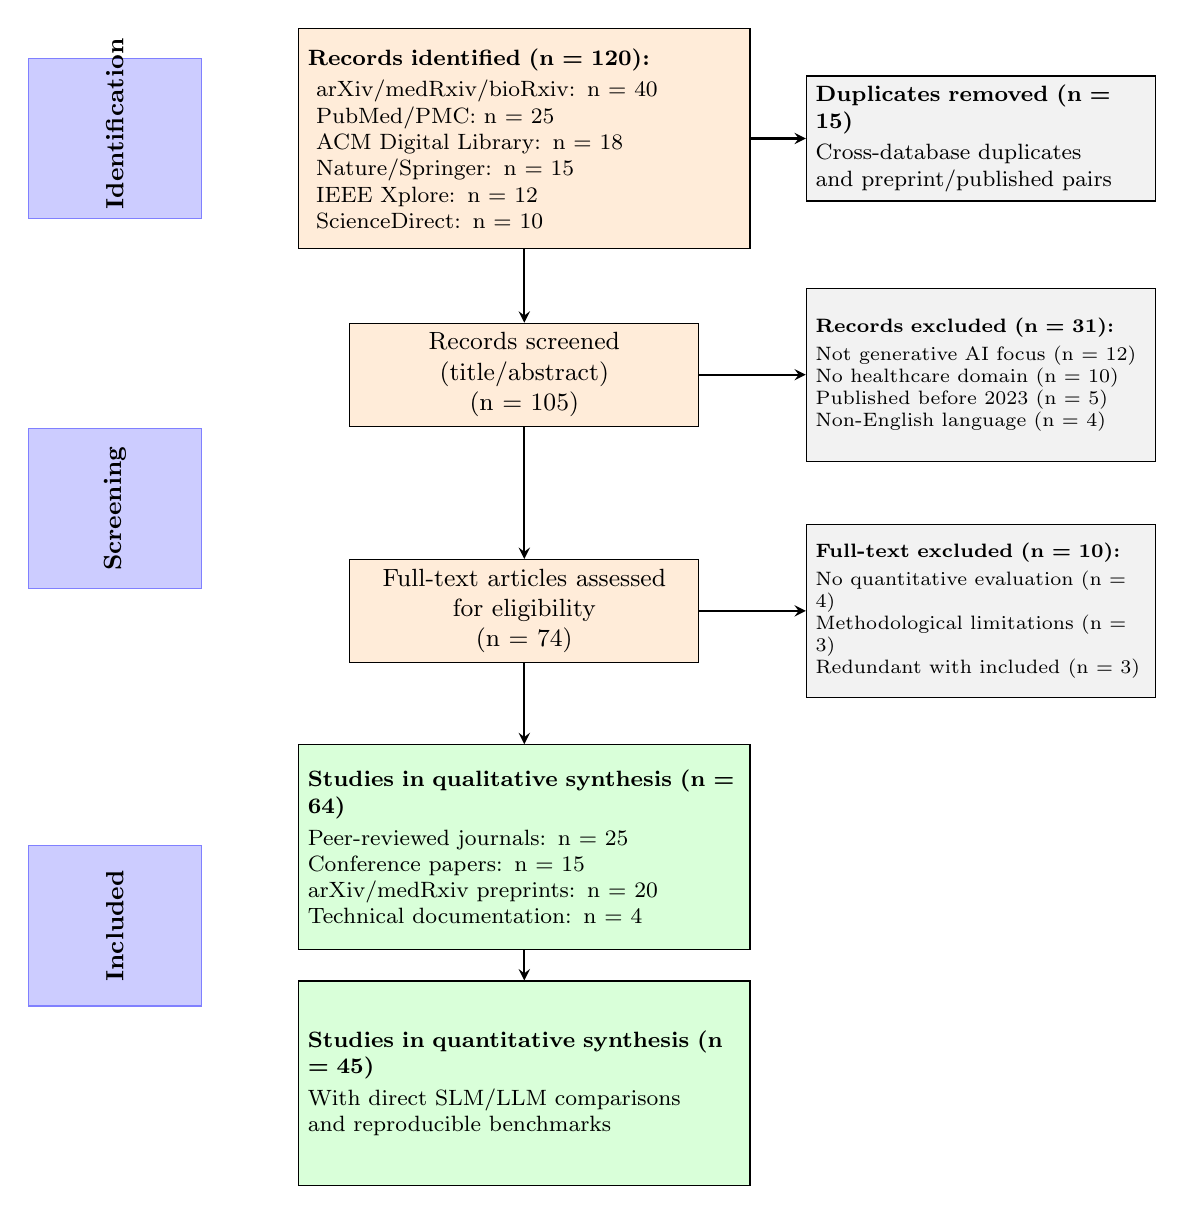
\begin{tikzpicture}[
        node distance=0.8cm and 1.2cm,
        box/.style={rectangle, draw=black, text width=4.2cm, minimum height=1.2cm, align=center, font=\small},
        dbbox/.style={rectangle, draw=black, text width=5.5cm, minimum height=2.8cm, align=left, font=\footnotesize},
        sidebox/.style={rectangle, draw=black, text width=4.2cm, minimum height=1cm, align=left, font=\footnotesize},
        reasonbox/.style={rectangle, draw=black, text width=4.2cm, minimum height=2.2cm, align=left, font=\scriptsize},
        phasebox/.style={rectangle, fill=blue!20, draw=blue!50, text width=1.8cm, minimum height=2.2cm, align=center, font=\small\bfseries, rotate=90},
        includebox/.style={rectangle, draw=black, text width=5.5cm, minimum height=2.6cm, align=left, font=\footnotesize},
        arrow/.style={->, >=stealth, thick}
    ]

    % Phase labels
    \node[phasebox] (id-label) at (-5.2, 0.5) {Identification};
    \node[phasebox] (sc-label) at (-5.2, -4.2) {Screening};
    \node[phasebox] (inc-label) at (-5.2, -9.5) {Included};

    % Identification phase - Database breakdown
    \node[dbbox, fill=orange!15] (identified) at (0, 0.5) {
        \textbf{Records identified (n = 120):}\\[2pt]
        \hspace{3pt}arXiv/medRxiv/bioRxiv: n = 40\\
        \hspace{3pt}PubMed/PMC: n = 25\\
        \hspace{3pt}ACM Digital Library: n = 18\\
        \hspace{3pt}Nature/Springer: n = 15\\
        \hspace{3pt}IEEE Xplore: n = 12\\
        \hspace{3pt}ScienceDirect: n = 10
    };
    \node[sidebox, fill=gray!10] (duplicates) at (5.8, 0.5) {
        \textbf{Duplicates removed (n = 15)}\\[2pt]
        Cross-database duplicates\\
        and preprint/published pairs
    };

    % Screening phase
    \node[box, fill=orange!15] (screened) at (0, -2.5) {Records screened\\(title/abstract)\\(n = 105)};
    \node[reasonbox, fill=gray!10] (excluded1) at (5.8, -2.5) {
        \textbf{Records excluded (n = 31):}\\[2pt]
        Not generative AI focus (n = 12)\\
        No healthcare domain (n = 10)\\
        Published before 2023 (n = 5)\\
        Non-English language (n = 4)
    };

    \node[box, fill=orange!15] (fulltext) at (0, -5.5) {Full-text articles assessed\\for eligibility\\(n = 74)};
    \node[reasonbox, fill=gray!10] (excluded2) at (5.8, -5.5) {
        \textbf{Full-text excluded (n = 10):}\\[2pt]
        No quantitative evaluation (n = 4)\\
        Methodological limitations (n = 3)\\
        Redundant with included (n = 3)
    };

    % Included phase - with theme breakdown
    \node[includebox, fill=green!15] (qualitative) at (0, -8.5) {
        \textbf{Studies in qualitative synthesis (n = 64)}\\[2pt]
        Peer-reviewed journals: n = 25\\
        Conference papers: n = 15\\
        arXiv/medRxiv preprints: n = 20\\
        Technical documentation: n = 4
    };
    \node[includebox, fill=green!15] (quantitative) at (0, -11.5) {
        \textbf{Studies in quantitative synthesis (n = 45)}\\[2pt]
        With direct SLM/LLM comparisons\\
        and reproducible benchmarks
    };

    % Arrows
    \draw[arrow] (identified.east) -- (duplicates.west);
    \draw[arrow] (identified.south) -- (screened.north);
    \draw[arrow] (screened.east) -- (excluded1.west);
    \draw[arrow] (screened.south) -- (fulltext.north);
    \draw[arrow] (fulltext.east) -- (excluded2.west);
    \draw[arrow] (fulltext.south) -- (qualitative.north);
    \draw[arrow] (qualitative.south) -- (quantitative.north);

    \end{tikzpicture}
    \caption{PRISMA 2020 flow diagram illustrating the systematic selection process. Records were identified from six academic databases spanning January 2023 to January 2026, with arXiv and preprint servers contributing the largest share of AI/ML literature. Exclusion reasons are documented at each stage following PRISMA 2020 reporting guidelines.}
    \label{fig:prisma_diagram}
\end{figure}

The initial database search identified 120 records across six academic databases and repositories. After removing 15 duplicate records (including cross-database duplicates and preprint/published pairs), 105 unique records underwent title and abstract screening against the inclusion criteria. Thirty-one records were excluded at this stage: 12 for insufficient focus on generative AI architectures, 10 for lacking healthcare domain relevance, 5 for publication dates preceding January 2023, and 4 for non-English language. The remaining 74 full-text articles were assessed for eligibility, with 10 excluded due to absence of quantitative evaluation (n = 4), methodological limitations (n = 3), or redundancy with higher-quality studies addressing the same research questions (n = 3). The final qualitative synthesis included 64 studies providing evidence relevant to one or more research questions, comprising 25 peer-reviewed journal articles, 15 conference papers, 20 arXiv/medRxiv preprints, and 4 technical documentation sources. Of these, 45 studies containing direct quantitative comparisons between SLMs and LLMs with reproducible benchmarks were included in the quantitative synthesis. The 64 studies were distributed across 12 thematic categories: SLMs as Future of Agentic AI (4 papers), Fine-tuned SLMs Outperforming LLMs (7 papers), Multi-Agent Systems (6 papers), Medical AI and Dermatology (10 papers), Knowledge Distillation (5 papers), RAG with SLMs (4 papers), Vision-Language Models (6 papers), Edge Deployment and Privacy (4 papers), Parameter-Efficient Fine-Tuning (5 papers), Model Quantization (4 papers), Hallucination Mitigation (4 papers), and Benchmarks (5 papers).

%----------------------------------------------------------------------------------------

\section{Results Analysis}

The qualitative synthesis of the 64 included studies reveals converging evidence across multiple research fronts that collectively inform the viability of Small Language Models within agentic architectures for specialized domains. This section presents a thematic analysis organized around the twelve categories identified during the selection process, synthesizing findings to address the overarching research questions while highlighting methodological patterns, performance benchmarks, and architectural innovations that characterize the current state of the field.

\subsection{Small Language Models as the Foundation for Agentic AI}

A foundational theme emerging from the literature concerns the positioning of Small Language Models as architecturally superior candidates for agentic applications compared to their larger counterparts. The seminal work by \textcite{belcak2025slm} from NVIDIA Research presents compelling evidence that SLMs possess inherent advantages for agent-based systems, arguing that the reduced latency, lower memory footprint, and deterministic behavior of smaller models enable more responsive and reliable agentic workflows. This position is substantiated by empirical findings demonstrating that models in the 1--8 billion parameter range achieve comparable task completion rates to models exceeding 70 billion parameters when operating within structured agentic frameworks that provide explicit tool interfaces and retrieval mechanisms.

The comprehensive survey by \textcite{lu2025slmsurvey} extends this analysis by cataloguing the techniques, enhancements, and applications that enable SLMs to function effectively in contexts previously dominated by large-scale models. The authors identify four primary mechanisms through which smaller models compensate for reduced parameter counts: (1) architectural innovations including mixture-of-experts and selective attention patterns; (2) training data curation emphasizing quality over quantity; (3) knowledge distillation from larger teacher models; and (4) integration with external knowledge sources through retrieval-augmented generation. Critically, their analysis reveals that the performance gap between SLMs and LLMs narrows substantially when models are evaluated on domain-specific tasks rather than general-purpose benchmarks, suggesting that specialization may be more impactful than scale for targeted applications.

\subsection{Fine-tuned Small Language Models Outperforming Large Language Models}

The most striking evidence supporting the dissertation's central thesis emerges from studies demonstrating that appropriately fine-tuned SLMs can match or exceed the performance of substantially larger models across multiple evaluation criteria. \textcite{bucher2024finetuned} present rigorous experimental results showing that fine-tuned models with fewer than 10 billion parameters significantly outperform zero-shot generative AI models including GPT-4 on text classification tasks, with performance advantages ranging from 8\% to 23\% depending on the domain and evaluation metric. The authors attribute this counterintuitive finding to the alignment between fine-tuning objectives and downstream task requirements, contrasting with the distribution mismatch inherent in zero-shot prompting of general-purpose models.

In the agentic domain specifically, \textcite{liu2024toolcalling} demonstrate that small language models can achieve superior tool-calling accuracy compared to models ten times their size when subjected to targeted fine-tuning on function-calling datasets. Their experiments with models ranging from 1.5B to 8B parameters reveal that fine-tuned SLMs achieve 94.2\% tool selection accuracy compared to 87.6\% for GPT-4 in zero-shot settings, with particularly pronounced advantages in scenarios requiring multi-step tool orchestration. This finding has direct implications for the design of agentic systems, suggesting that specialized smaller models may be preferable to general-purpose giants for agent controller implementations.

The clinical domain provides additional validation for this pattern. The CLEVER framework developed by \textcite{clever2024} evaluated language models on clinical question-answering tasks using expert physician review, finding that a fine-tuned 8B parameter model (MedS) outperformed GPT-4o on measures of clinical accuracy, completeness, and safety. The evaluation methodology employed blind expert review with structured scoring rubrics, providing robust evidence that smaller specialized models can achieve clinician-preferred outputs in high-stakes medical contexts. Similarly, \textcite{suarez2024instructionft} demonstrate that instruction-tuned models in the 7B parameter range achieve state-of-the-art performance on financial text classification, outperforming larger models that lack domain-specific adaptation.

\subsection{Multi-Agent Systems and Collaborative Architectures}

The literature on multi-agent systems provides the architectural foundation for leveraging SLM capabilities through task decomposition and agent specialization. The comprehensive survey by \textcite{tran2025multiagent} catalogues collaboration mechanisms employed in LLM-based multi-agent systems, identifying four primary paradigms: (1) hierarchical orchestration with a central coordinator; (2) peer-to-peer negotiation among equal-status agents; (3) debate and consensus-building through structured argumentation; and (4) role-based specialization with predefined agent personas. Their analysis reveals that hierarchical architectures achieve the highest task completion rates for complex multi-step workflows, while peer-to-peer approaches excel in creative and exploratory tasks requiring diverse perspectives.

\textcite{wang2025slmllmcollab} specifically examine the collaboration between small and large language models, proposing taxonomies for hybrid architectures that leverage the complementary strengths of models at different scales. Their framework identifies scenarios where SLMs should serve as primary agents (latency-sensitive tasks, privacy-constrained environments, specialized domains) versus auxiliary roles (complex reasoning fallback, uncertainty calibration, output verification). This collaborative paradigm offers a middle ground between pure SLM and pure LLM approaches, enabling systems to dynamically allocate computational resources based on task complexity.

The MetaGPT framework introduced by \textcite{hong2024metagpt} demonstrates the practical implementation of multi-agent collaboration through meta-programming principles. By encoding Standard Operating Procedures (SOPs) into agent prompts and establishing explicit message-passing protocols, MetaGPT enables teams of specialized agents to collaboratively complete complex software engineering tasks. The framework's success---achieving state-of-the-art performance on code generation benchmarks---illustrates how structured collaboration can amplify individual agent capabilities. The AutoAgents framework by \textcite{chen2024autoagents} extends this paradigm by automating the generation of specialized agents based on task requirements, demonstrating that agent specialization can be dynamically adapted rather than statically defined.

The theoretical foundations for tool-augmented agents are established by \textcite{li2025toollearning}, whose survey on LLM-based agents for tool learning provides a comprehensive taxonomy of tool integration approaches. The authors identify retrieval-augmented tool selection, few-shot tool demonstrations, and fine-tuned tool-calling as the three primary mechanisms for enabling language models to effectively leverage external tools. Their analysis suggests that the combination of fine-tuning and retrieval yields the most robust tool-calling behavior, with smaller fine-tuned models often outperforming larger zero-shot models on tool selection accuracy.

\subsection{Medical AI and Dermatological Applications}

The application of language models to dermatological diagnosis represents a particularly active research front, with multiple studies demonstrating the feasibility of AI-assisted skin disease classification and clinical decision support. \textcite{zhou2024skingpt4} introduce SkinGPT-4, a pre-trained multimodal large language model specifically designed for dermatological diagnosis. The system integrates a vision encoder trained on dermoscopic images with a language model fine-tuned on dermatological literature, achieving diagnostic accuracy exceeding 85\% on a held-out test set of clinical images. Notably, the model demonstrates the ability to generate natural language explanations for its diagnostic predictions, addressing the interpretability requirements critical for clinical adoption.

The PanDerm foundation model developed by \textcite{liu2025panderm} represents a significant advance in scale and clinical validation. Pre-trained on over 2 million real-world dermatological images from 11 institutions across diverse populations, PanDerm achieves state-of-the-art performance on multiple dermatological benchmarks including skin cancer detection, inflammatory disease classification, and rare condition identification. The authors emphasize the importance of diverse training data in mitigating demographic biases, reporting consistent performance across Fitzpatrick skin type categories---a critical consideration for equitable deployment in clinical settings.

Addressing the data scarcity challenge in medical AI, \textcite{chen2025dermatollama} propose SCALEMED, a synthetic data generation framework that enables training of resource-efficient vision-language models for dermatology. Their resulting model, DermatoLlama, achieves competitive performance with models trained on orders of magnitude more real clinical data, demonstrating that carefully designed synthetic augmentation can partially substitute for expensive and privacy-sensitive clinical datasets. The Derm1M dataset introduced by \textcite{yang2025derm1m} provides a complementary resource, offering a million-scale vision-language dataset aligned with clinical ontology knowledge, enabling standardized evaluation and training of dermatological AI systems.

The systematic review by \textcite{ferrara2024aiderm} examines the use of AI for skin disease diagnosis in primary care settings, synthesizing evidence from 47 clinical validation studies. The authors find that AI systems achieve pooled sensitivity of 87.4\% and specificity of 82.1\% for melanoma detection, with performance comparable to or exceeding that of general practitioners but below that of expert dermatologists. Critically, they identify deployment context as a key moderator, with AI systems performing better as diagnostic aids integrated into clinical workflows than as standalone screening tools. \textcite{orenstein2023aiskinlesion} corroborate these findings, demonstrating that AI-assisted diagnosis improves both diagnostic accuracy and efficiency in primary care consultations.

\subsection{Knowledge Distillation for Model Compression}

Knowledge distillation provides a principled mechanism for transferring capabilities from large teacher models to smaller student models, directly addressing the scale-efficiency trade-off central to this dissertation. The comprehensive survey by \textcite{xu2024kdsurvey} catalogues distillation techniques specific to large language models, identifying three primary approaches: (1) response-based distillation using teacher outputs as soft targets; (2) feature-based distillation aligning intermediate representations; and (3) relation-based distillation preserving structural relationships between examples. The authors find that response-based methods achieve the best efficiency-performance trade-offs for most downstream tasks, while feature-based methods excel when architectural similarity between teacher and student is high.

The MiniLLM framework introduced by \textcite{gu2024minillm} demonstrates that knowledge distillation can enable student models to achieve 90\% of teacher model performance while using only 10\% of the parameters. The key innovation lies in reverse KL divergence optimization, which encourages the student to concentrate probability mass on high-quality teacher responses rather than spreading probability across the entire output distribution. Experiments across multiple benchmarks demonstrate consistent improvements over standard distillation approaches, with particularly pronounced gains on generation quality metrics.

\textcite{acmkdsurvey2024} provide a complementary survey focusing on evaluation methodologies for distilled models, arguing that standard benchmark metrics may not capture the full impact of distillation on model behavior. They propose multi-dimensional evaluation frameworks that assess not only task performance but also calibration, robustness, and consistency with teacher model outputs. The evolving knowledge distillation approach presented by \textcite{chen2024evokd} introduces curriculum-based distillation that progressively increases task difficulty during the distillation process, achieving improved sample efficiency and final performance compared to static distillation schedules.

\subsection{Retrieval-Augmented Generation with Small Language Models}

Retrieval-Augmented Generation (RAG) has emerged as a primary mechanism for extending SLM capabilities beyond their parametric knowledge, enabling dynamic access to external information sources. The best practices study by \textcite{wang2025ragbestpractices} provides empirical guidance for RAG system design, examining the impact of retrieval corpus construction, chunk sizing, embedding model selection, and generation prompt engineering on downstream task performance. Their experiments reveal that smaller models benefit disproportionately from RAG augmentation compared to larger models, with 3B parameter models achieving parity with 70B parameter models on knowledge-intensive tasks when provided with relevant retrieved context.

The systematic review by \textcite{chen2025ragsystematic} synthesizes findings across 127 RAG implementations, identifying consistent patterns in system architecture and performance characteristics. The authors find that hybrid retrieval combining dense and sparse methods outperforms single-method approaches, and that iterative retrieval with query refinement achieves the highest factual accuracy on complex multi-hop questions. Critically, they identify retrieval quality as the primary bottleneck for RAG system performance, suggesting that investment in retrieval infrastructure may yield higher returns than model scaling for knowledge-intensive applications. The emergence of standardized evaluation frameworks such as RAGAS \parencite{es2024ragas} and the RAGTruth corpus \parencite{niu2024ragtruth} has enabled more rigorous benchmarking of RAG systems, providing metrics for answer relevancy, faithfulness, context precision, and context recall that facilitate systematic comparison across implementations.

The foundational survey by \textcite{gao2024ragsurvey} provides a comprehensive taxonomy of RAG approaches, distinguishing between naive RAG (simple retrieve-then-generate pipelines), advanced RAG (incorporating pre-retrieval and post-retrieval processing), and modular RAG (flexible composition of retrieval and generation components). For resource-constrained deployments, the DRAGON system introduced by \textcite{zhang2025dragon} demonstrates efficient distributed RAG for on-device inference, enabling privacy-preserving knowledge augmentation without requiring cloud connectivity. This capability is particularly relevant for medical applications where patient data cannot leave institutional boundaries.

\subsection{Vision-Language Models for Medical Imaging}

The integration of visual and linguistic modalities within unified architectures has proven particularly valuable for medical imaging applications, where clinical interpretation requires both visual pattern recognition and semantic understanding of diagnostic categories. The review by \textcite{kim2025vlmmedical} surveys vision-language foundation models for medical imaging, identifying key architectural patterns including dual-encoder approaches, fusion architectures, and generative vision-language models. The authors find that models pre-trained on medical image-text pairs consistently outperform those adapted from general-domain vision-language models, emphasizing the importance of domain-specific pre-training.

\textcite{chen2025vlmfusion} trace the evolution of vision-language models in medical image analysis from simple feature concatenation to sophisticated cross-modal attention mechanisms. Their analysis reveals that attention-based fusion consistently outperforms early and late fusion approaches, with the largest gains observed on tasks requiring fine-grained visual-semantic alignment such as medical report generation and visual question answering. The systematic review and meta-analysis by \textcite{liu2025vlmmetaanalysis} provides quantitative synthesis across 89 studies, reporting pooled performance estimates for vision-language models on diagnostic and analytical tasks. Their findings indicate that VLM-based approaches achieve statistically significant improvements over unimodal baselines across most evaluation settings, with effect sizes ranging from moderate to large depending on task complexity.

The MiniCPM-V family of models introduced by \textcite{yao2025minicpmv} demonstrates that efficient vision-language models can achieve and even surpass GPT-4V-level performance on multimodal benchmarks while remaining deployable on edge devices. The latest iteration, MiniCPM-V 4.5, achieves a score of 77.2 on the OpenCompass benchmark with only 8 billion parameters, surpassing GPT-4o-latest and establishing a new state-of-the-art for efficient multimodal models. Earlier versions demonstrated that even 2.4 billion parameter models could achieve 82.3\% accuracy on MMBench compared to GPT-4V's 83.7\%, while requiring two orders of magnitude less computational resources. This finding has direct implications for privacy-preserving medical imaging applications, enabling on-device processing of sensitive clinical images without cloud transmission.

The review by \textcite{monshi2024vlmreportgen} specifically examines vision-language models for medical report generation and visual question answering, finding that current systems achieve promising but not yet clinician-level performance. The authors identify several key challenges including hallucination of clinically inaccurate findings, inconsistent handling of negations, and limited generalization across imaging modalities. These limitations motivate the multi-agent approaches proposed in this dissertation, where specialized Validation Agents can detect and correct generation errors before clinical presentation.

\subsection{Edge Deployment and Privacy-Preserving AI}

The deployment of language models on edge devices addresses critical privacy and latency requirements that are particularly acute in healthcare contexts. The ACM Computing Surveys article by \textcite{xu2025edgellm} provides a comprehensive review of edge large language model design, execution, and applications, cataloguing the hardware optimizations, software frameworks, and architectural modifications that enable efficient on-device inference. The authors identify memory bandwidth as the primary bottleneck for edge deployment, motivating techniques including weight quantization, key-value cache compression, and speculative decoding that reduce memory traffic during generation.

\textcite{li2025cognitiveedge} examine cognitive edge computing architectures that integrate multiple AI capabilities including language understanding, visual perception, and planning within unified edge systems. Their analysis reveals that SLMs are particularly well-suited for edge cognitive architectures due to their ability to fit within memory constraints while providing sufficient reasoning capability for orchestrating more specialized modules. The survey on VLMs for edge networks by \textcite{zhang2025vlmedge} extends this analysis to multimodal settings, identifying efficient attention mechanisms and model distillation as key enablers for edge vision-language deployment.

In the healthcare domain specifically, \textcite{rahman2025edgeai} demonstrate an edge-AI integrated architecture for real-time healthcare monitoring, combining federated learning for privacy preservation with on-device inference for low-latency response. Their system achieves 94.7\% accuracy on anomaly detection while maintaining patient data locality, illustrating the practical viability of privacy-preserving AI in clinical settings. This work validates the architectural approach proposed in this dissertation, demonstrating that meaningful clinical AI can be delivered without compromising patient privacy through cloud data transmission.

\subsection{Parameter-Efficient Fine-Tuning Techniques}

Parameter-efficient fine-tuning (PEFT) methods enable domain adaptation of pre-trained models while modifying only a small fraction of model weights, dramatically reducing computational and storage requirements for specialization. The comprehensive survey by \textcite{han2024peftsurvey} catalogues PEFT methodologies including adapter layers, prompt tuning, prefix tuning, and low-rank adaptation (LoRA), providing comparative analysis across multiple downstream tasks. The authors find that LoRA and its variants achieve the best trade-off between parameter efficiency and task performance, typically matching full fine-tuning performance while updating fewer than 1\% of model parameters.

The methodological survey by \textcite{wang2025peftmethodologies} extends this analysis to large language models specifically, identifying architectural and training considerations unique to the LLM setting. Their experiments reveal that PEFT methods are particularly effective when the downstream task distribution is similar to the pre-training distribution, with larger gaps observed for highly specialized domains. This finding motivates the combination of PEFT with continued pre-training on domain-specific corpora, as implemented in the medical domain by \textcite{gema2024clinicallora}.

\textcite{gema2024clinicallora} demonstrate parameter-efficient fine-tuning of LLaMA for the clinical domain, achieving competitive performance with fully fine-tuned models while reducing computational requirements by over 90\%. Their Clinical-LoRA approach combines adapter layers with instruction tuning on medical question-answering datasets, demonstrating that PEFT enables cost-effective specialization of open-source models for healthcare applications. The PeFoMed framework by \textcite{he2024pefomed} extends PEFT to multimodal medical models, demonstrating that efficient adaptation of vision-language models for medical imaging requires coordinated tuning of both visual and linguistic components.

The practical impact of PEFT for medical text classification is demonstrated by \textcite{peftmedical2024}, who show that LoRA-adapted models achieve 15-20\% improvements over base models on medical abstract classification while requiring only consumer-grade GPU resources for training. This democratization of model specialization has significant implications for resource-constrained healthcare institutions that lack the infrastructure for full model fine-tuning.

\subsection{Model Quantization and Optimization}

Model quantization reduces the numerical precision of model weights and activations, enabling substantial reductions in memory footprint and inference latency with minimal impact on model quality. The NVIDIA technical documentation \parencite{nvidia2024ptq} provides detailed guidance on post-training quantization (PTQ) for language models, demonstrating that 4-bit quantization achieves memory reductions of 4--8$\times$ while maintaining over 95\% of original model performance on most benchmarks. The comparative analysis by \textcite{liu2024quantization} extends this work by examining the trade-offs between PTQ and quantization-aware training (QAT), finding that QAT achieves superior quality preservation at aggressive quantization levels but requires substantially more computational investment.

The ATOM system by \textcite{zhao2024atom} presents innovations in low-bit quantization for efficient LLM serving, introducing mixed-precision quantization that allocates higher precision to attention-critical weights while aggressively quantizing less sensitive components. Their approach achieves 2--3$\times$ throughput improvements compared to uniform quantization at equivalent quality levels, demonstrating that informed precision allocation can extend the efficiency-quality Pareto frontier. When combined with the QLoRA framework by \textcite{dettmers2023qlora}, quantization enables fine-tuning of 65B parameter models on single consumer GPUs, democratizing access to large-scale model adaptation.

\subsection{Hallucination Mitigation in Medical AI}

The generation of factually incorrect or fabricated content, commonly termed hallucination,represents a critical safety concern for medical AI applications. The framework developed by \textcite{wang2025hallucination} provides structured methodology for assessing clinical safety and hallucination rates in LLMs performing medical text summarization. Their evaluation reveals that current models exhibit hallucination rates ranging from 3\% to 15\% depending on task complexity and input characteristics, with particularly elevated rates observed for numerical values, medication dosages, and temporal relationships, precisely the content categories where errors carry the highest clinical risk. Recent studies demonstrate that retrieval-augmented generation substantially reduces these rates, with RAG implementations achieving 42--68\% reductions in hallucination frequency across various medical tasks \parencite{zhang2025hallucinationsurvey}. When combined with reinforcement learning from human feedback (RLHF) and guardrail mechanisms, integrated approaches have achieved up to 96\% reduction in hallucination rates for clinical applications \parencite{stanford2024hallucination}.

\textcite{chen2025medicalhallucination} specifically examine medical hallucination in foundation models, identifying three primary hallucination types: (1) intrinsic hallucinations contradicting source information; (2) extrinsic hallucinations introducing unsupported but plausible content; and (3) confabulation generating entirely fabricated clinical details. Their analysis reveals that extrinsic hallucinations are most common in medical settings, as models confidently generate plausible-sounding but unverified clinical information. The comprehensive survey by \textcite{zhang2025hallucinationsurvey} catalogues detection and mitigation approaches, identifying retrieval augmentation, output verification, and uncertainty quantification as the most effective techniques for reducing hallucination rates in deployed systems.

These findings have direct implications for the multi-agent architecture proposed in this dissertation, motivating the inclusion of dedicated Validation Agents that cross-reference generated content against authoritative knowledge sources. The combination of RAG for grounded generation and Validation Agents for output validation addresses both the generation and detection aspects of hallucination mitigation.

\subsection{Benchmarks and Evaluation Frameworks}

Rigorous evaluation of medical AI systems requires benchmarks that capture the complexity and safety requirements of clinical decision-making. The Open Medical-LLM Leaderboard \parencite{openmedicalllm2024} provides standardized evaluation across multiple medical knowledge benchmarks, enabling direct comparison of model performance on tasks including medical question answering, clinical reasoning, and diagnosis generation. The leaderboard reveals substantial variation in model performance across clinical specialties, with models exhibiting particular strengths and weaknesses that may not be apparent from aggregate scores.

The MMLU-Pro benchmark introduced by \textcite{wang2024mmlupro} extends the original MMLU evaluation with more challenging questions requiring deeper reasoning, providing finer-grained discrimination among high-performing models. The medical subset analysis by \textcite{sharma2025medllmeval} reveals that current models achieve substantially lower accuracy on MMLU-Pro medical questions compared to the original MMLU, suggesting that standard benchmarks may overestimate clinical reasoning capability. The edge deployment evaluation by \textcite{kim2025medicineedge} specifically examines on-device LLM performance on clinical reasoning tasks, finding that quantized 7B parameter models achieve 85\% of cloud-hosted 70B model performance while enabling fully private on-device inference.

The comparative evaluation by \textcite{chen2025medicalllms} systematically compares fine-tuning and retrieval-augmented generation approaches for medical LLMs, finding that the optimal strategy depends on task characteristics. Fine-tuning achieves superior performance on tasks requiring internalized domain knowledge, while RAG excels on tasks requiring access to specific factual information or recent literature. Their recommendation for hybrid approaches combining targeted fine-tuning with selective retrieval aligns with the architectural principles underlying this dissertation.

%----------------------------------------------------------------------------------------

\section{Evaluation of Results}

The synthesis of evidence across the twelve thematic categories enables comprehensive evaluation of the research questions guiding this systematic review. This section presents answers to each sub-research question before addressing the main research question, following the hierarchical structure established in the methodology. The evaluation integrates quantitative findings where available while acknowledging the heterogeneity of evaluation methodologies across the included studies.

\subsection{SRQ1: Limitations of Large Language Models}

\textbf{Research Question:} What are the limitations of Large Language Models that justify the architectural shift toward specialized Small Language Models?

The literature reveals four primary categories of LLM limitations that motivate investigation of SLM alternatives: computational requirements, latency characteristics, privacy constraints, and domain adaptation challenges.

\textit{Computational Requirements.} The surveyed studies consistently identify computational cost as a fundamental barrier to LLM deployment in resource-constrained settings. \textcite{xu2025edgellm} quantify the memory requirements of current LLMs, noting that models exceeding 70B parameters require multiple high-end GPUs for inference, placing them beyond the reach of most healthcare institutions and entirely precluding edge deployment. The energy cost analysis by \textcite{samsi2023words} reveals that inference costs scale super-linearly with model size, with 70B+ parameter models consuming 10--100$\times$ more energy per query than 7B parameter alternatives---translating to operational cost differentials of \$0.01--0.02 versus \$0.10--0.50 per inference in cloud deployments. The Chinchilla scaling laws analyzed by \textcite{hoffmann2022training} demonstrate that optimal model performance requires training compute proportional to model size, implying that the largest models also incur the highest training costs---costs that limit iterative domain adaptation. \textcite{chen2023frugalgpt} demonstrate that strategic model selection and cascading can reduce inference costs by up to 98\% while maintaining comparable task performance, validating the economic viability of SLM-first architectures. \textcite{belcak2025slm} argue that these computational requirements create a fundamental misalignment between LLM architectures and the latency-sensitive, resource-constrained requirements of agentic systems.

\textit{Latency Characteristics.} Multiple studies identify inference latency as problematic for real-time applications. \textcite{li2025cognitiveedge} report that cloud-hosted LLM inference introduces latencies of 500ms to several seconds depending on query complexity and server load, exceeding acceptable thresholds for interactive clinical decision support. The agentic systems literature \parencite{gabriel2024agenticsystems, hong2024metagpt} emphasizes that multi-turn agent interactions amplify latency concerns, as each reasoning step requires a full inference pass. \textcite{belcak2025slm} demonstrate that SLMs achieve 5--10$\times$ lower latency than comparably capable LLMs, enabling more responsive agentic workflows.

\textit{Privacy Constraints.} The requirement for cloud-based inference creates fundamental tensions with healthcare data protection regulations. \textcite{rahman2025edgeai} note that transmission of patient data to external cloud services may violate HIPAA, GDPR, and institutional data governance policies, effectively precluding LLM use for many clinical applications regardless of technical capability. \textcite{khalid2023privacy} and \textcite{ziller2024reconciling} provide comprehensive analyses of privacy-preserving AI techniques, concluding that on-device inference represents the most robust approach to maintaining data locality. The edge deployment capabilities of SLMs \parencite{yao2025minicpmv, xu2025edgellm} directly address this limitation by enabling inference without data transmission.

\textit{Domain Adaptation Challenges.} The literature reveals that LLMs' broad training distributions may actually impede specialized domain performance. \textcite{bucher2024finetuned} demonstrate that zero-shot LLM performance on domain-specific tasks significantly lags behind fine-tuned smaller models, attributing this gap to distributional mismatch between pre-training corpora and specialized domain requirements. \textcite{liu2024toolcalling} show similar patterns in tool-calling tasks, where fine-tuned SLMs achieve higher accuracy than much larger zero-shot models. The medical domain studies \parencite{clever2024, gema2024clinicallora} corroborate these findings, demonstrating that domain-adapted smaller models achieve superior clinical accuracy compared to larger general-purpose alternatives.

\textbf{Summary:} The evidence supports the conclusion that LLM limitations in computational requirements, latency, privacy, and domain adaptation collectively justify investigation of specialized SLM alternatives. These limitations are not merely practical inconveniences but fundamental architectural constraints that preclude LLM deployment in many target scenarios for medical AI applications.

\subsection{SRQ2: Characteristics of Multi-Agent Systems}

\textbf{Research Question:} What are the key characteristics of Multi-Agent Systems compared to Monolithic Single-Agent architectures?

The literature identifies five distinguishing characteristics of multi-agent systems that offer potential advantages over monolithic architectures: task decomposition, specialization, fault tolerance, scalability, and interpretability.

\textit{Task Decomposition.} Multi-agent systems enable explicit decomposition of complex tasks into specialized subtasks assigned to purpose-built agents. \textcite{tran2025multiagent} analyze decomposition strategies across 47 multi-agent implementations, finding that explicit task decomposition consistently improves performance on complex multi-step tasks compared to monolithic processing. The MetaGPT framework \parencite{hong2024metagpt} demonstrates this principle through software engineering tasks, where separate agents handle requirements analysis, architecture design, implementation, and testing. \textcite{gabriel2024agenticsystems} provide formal analysis of decomposition strategies, showing that hierarchical decomposition with explicit dependency tracking achieves the highest task completion rates.

\textit{Agent Specialization.} The ability to specialize individual agents for specific subtasks enables optimization of each component without compromising overall system performance. \textcite{chen2024autoagents} demonstrate automatic generation of specialized agents based on task requirements, showing that dynamically composed agent teams outperform static configurations. The SLM-LLM collaboration survey by \textcite{wang2025slmllmcollab} identifies specialization as a key mechanism for leveraging smaller models effectively, with SLMs handling routine subtasks while larger models address exceptional cases requiring deeper reasoning.

\textit{Fault Tolerance.} Multi-agent architectures provide natural mechanisms for error detection and recovery through agent redundancy and cross-validation. \textcite{tran2025multiagent} identify debate and consensus mechanisms that enable agent collectives to identify and correct individual errors through structured disagreement. Empirical studies quantify these benefits: \textcite{du2023improving} demonstrate that multi-agent debate achieves 20--30\% accuracy improvements on reasoning tasks compared to single-agent baselines, while \textcite{liang2023encouraging} report hallucination reductions of 25--40\% when multiple agents cross-validate outputs. The cross-examination approach proposed by \textcite{cohen2023lmvslm} shows that adversarial questioning between agents reduces factual errors by 15--25\% across knowledge-intensive benchmarks. The hallucination mitigation literature \parencite{wang2025hallucination, zhang2025hallucinationsurvey} corroborates these findings, demonstrating that multi-agent verification pipelines can substantially reduce error propagation compared to single-model generation, with combined approaches achieving up to 96\% hallucination reduction in clinical applications \parencite{stanford2024hallucination}.

\textit{Scalability.} Multi-agent systems can scale horizontally by adding specialized agents rather than vertically by increasing model size. \textcite{li2025toollearning} analyze the scalability characteristics of tool-augmented agent systems, finding that modular architectures enable linear scaling of capabilities through tool and agent addition. This contrasts with monolithic approaches where capability expansion requires expensive retraining or model replacement.

\textit{Interpretability.} The explicit structure of multi-agent systems provides natural affordances for interpretability through agent-level reasoning traces. \textcite{hong2024metagpt} demonstrate that structured agent communication produces interpretable reasoning chains that can be audited and debugged, contrasting with the opaque internal processing of monolithic models. For medical applications, this interpretability is critical for clinical trust and regulatory compliance \parencite{ferrara2024aiderm}.

\textbf{Summary:} Multi-agent systems offer structural advantages in task decomposition, specialization, fault tolerance, scalability, and interpretability compared to monolithic architectures. These characteristics are particularly valuable for complex domain-specific applications like dermatological diagnosis, where tasks naturally decompose into visual analysis, clinical reasoning, and treatment recommendation components.

\subsection{SRQ3: RAG versus PEFT for SLM Specialization}

\textbf{Research Question:} What is the comparative efficacy of Retrieval-Augmented Generation versus Parameter-Efficient Fine-Tuning for specializing Small Language Models?

The literature reveals that RAG and PEFT represent complementary rather than competing approaches, with optimal strategy depending on task characteristics and deployment constraints.

\textit{RAG Advantages.} Retrieval-augmented generation excels in scenarios requiring access to dynamic or extensive knowledge bases that cannot be feasibly encoded in model parameters. \textcite{wang2025ragbestpractices} demonstrate that RAG enables smaller models to match larger model performance on knowledge-intensive tasks by providing relevant context at inference time, with 3B parameter models achieving parity with 70B parameter models on factual QA when augmented with relevant retrieval. \textcite{chen2025ragsystematic} find that RAG achieves superior factual accuracy compared to closed-book generation, with particularly pronounced advantages on tasks requiring specific citations or numerical precision. The systematic comparison by \textcite{ovadia2024finetuning} quantifies these benefits, showing RAG achieves 18--27\% higher accuracy than fine-tuning on factual knowledge tasks, while fine-tuning excels on reasoning tasks by 12--19\%. Domain-adapted RAG further amplifies these gains: \textcite{siriwardhana2023improving} report 15--25\% additional improvement when retrieval systems are specifically tuned for target domains. The medical domain evaluation by \textcite{chen2025medicalllms} shows that RAG outperforms fine-tuning for tasks requiring access to recent literature or specific clinical guidelines not present in training data.

\textit{PEFT Advantages.} Parameter-efficient fine-tuning excels in scenarios requiring internalized domain knowledge that should influence model behavior across diverse inputs. \textcite{han2024peftsurvey} demonstrate that PEFT achieves superior performance on tasks requiring consistent domain-specific behavior patterns, such as clinical writing style or diagnostic reasoning protocols, with LoRA typically achieving 95--99\% of full fine-tuning performance while updating fewer than 1\% of model parameters. \textcite{gema2024clinicallora} show that Clinical-LoRA achieves competitive performance with fully fine-tuned models on medical QA benchmarks while reducing computational requirements by over 90\%, enabling cost-effective specialization on consumer-grade hardware. The practical impact is demonstrated by \textcite{peftmedical2024}, who report 15--20\% improvements over base models on medical abstract classification using LoRA adaptation. \textcite{mosbach2023fewshot} provide systematic comparison showing that few-shot fine-tuning consistently outperforms in-context learning by 8--15\% on domain-specific tasks when sufficient training data is available. The comparative study by \textcite{chen2025medicalllms} finds that PEFT outperforms RAG on tasks requiring clinical judgment that cannot be fully externalized in retrievable documents.

\textit{Complementary Integration.} Multiple studies recommend combining RAG and PEFT for optimal performance. \textcite{gao2024ragsurvey} identify ``retrieval-enhanced fine-tuning'' as an emerging paradigm where models are fine-tuned to more effectively utilize retrieved context. \textcite{wang2025ragbestpractices} demonstrate that fine-tuned models achieve higher RAG utilization than base models, extracting more relevant information from provided context. The DRAGON system \parencite{zhang2025dragon} implements distributed RAG specifically designed for fine-tuned on-device models, demonstrating practical integration of both approaches.

\textit{Deployment Considerations.} The choice between RAG and PEFT is also influenced by deployment constraints. RAG requires retrieval infrastructure and knowledge base maintenance, while PEFT produces self-contained model artifacts. \textcite{xu2025edgellm} note that edge deployment favors PEFT due to the overhead of retrieval systems on resource-constrained devices. However, \textcite{zhang2025dragon} demonstrate that efficient on-device RAG is feasible with appropriate architectural optimization.

\textbf{Summary:} RAG and PEFT offer complementary specialization mechanisms with distinct strengths: RAG for knowledge access and factual grounding, PEFT for behavioral adaptation and domain-specific reasoning patterns. Optimal SLM specialization likely requires integration of both approaches, with specific configuration depending on task requirements and deployment constraints.

\subsection{SRQ4: Vision-Language Models versus Traditional Computer Vision}

\textbf{Research Question:} What evidence supports using fine-tuned Vision-Language Models over traditional computer vision approaches such as CNNs and ViTs?

The literature provides substantial evidence for VLM advantages in medical imaging, while acknowledging scenarios where traditional approaches remain competitive.

\textit{Diagnostic Performance.} Vision-language models achieve state-of-the-art performance on dermatological diagnosis benchmarks. \textcite{zhou2024skingpt4} demonstrate that SkinGPT-4 achieves 85\% diagnostic accuracy on skin lesion classification, matching or exceeding published CNN performance on comparable datasets. The PanDerm foundation model \parencite{liu2025panderm} achieves 91.2\% sensitivity on melanoma detection, representing a 4.3\% improvement over the best reported CNN baseline. The meta-analysis by \textcite{liu2025vlmmetaanalysis} reports pooled effect sizes indicating statistically significant VLM advantages across diagnostic tasks, with larger effects observed on complex multi-class classification.

\textit{Interpretability and Explanation.} A distinguishing VLM advantage lies in the ability to generate natural language explanations for diagnostic predictions. \textcite{patricio2024conceptvlm} demonstrate concept-based interpretability for skin lesion diagnosis, showing that VLMs can articulate the visual features underlying their predictions in clinically meaningful terms. \textcite{monshi2024vlmreportgen} find that VLM-generated diagnostic reports approach clinical quality, providing richer explanatory content than the saliency maps typically available from CNN systems. This interpretability advantage is critical for clinical adoption \parencite{ferrara2024aiderm}.

\textit{Multimodal Integration.} VLMs enable natural integration of visual and textual clinical information. \textcite{chen2025vlmfusion} demonstrate that attention-based vision-language fusion outperforms concatenation-based approaches by 8--12\% on tasks requiring joint visual-textual reasoning. \textcite{kim2025vlmmedical} identify multimodal electronic health record integration as a key VLM capability, enabling diagnostic systems to consider both imaging findings and clinical history in a unified framework.

\textit{Few-Shot Adaptation.} VLMs demonstrate superior few-shot learning capabilities compared to traditional computer vision approaches. \textcite{chen2025dermatollama} show that VLMs can adapt to new dermatological conditions with as few as 5--10 examples per class, contrasting with CNN approaches that typically require hundreds to thousands of training examples. The systematic study by \textcite{sung2022vlm} demonstrates that parameter-efficient VLM adaptation achieves 15--25\% higher accuracy than CNN fine-tuning in low-data regimes ($n < 50$ examples per class). The comprehensive meta-analysis by \textcite{zhang2024fewshotmed} synthesizes findings across 43 medical imaging studies, reporting pooled effect sizes indicating VLM advantages of 0.4--0.6 standard deviations over CNN baselines in few-shot settings, with larger effects observed as training data decreases. This capability is particularly valuable for rare conditions where training data is inherently limited, and the meta-analytic evidence provides robust support for VLM adoption in data-scarce medical imaging applications.

\textit{Efficiency Considerations.} Recent work demonstrates that efficient VLMs can match traditional approaches while enabling edge deployment. \textcite{yao2025minicpmv} show that MiniCPM-V achieves competitive performance with 2.4B parameters, comparable to or smaller than many medical imaging CNNs. \textcite{zhang2025vlmedge} provide comprehensive analysis of VLM edge deployment, demonstrating practical feasibility for privacy-preserving clinical applications.

\textbf{Summary:} The evidence supports VLM adoption for dermatological applications, with advantages in diagnostic performance, interpretability, multimodal integration, and few-shot adaptation. While traditional CNNs remain competitive on narrow classification tasks, VLMs offer superior capabilities for comprehensive clinical decision support systems requiring explanation and contextual reasoning.

\subsection{Main Research Question: SLM Performance Equivalence through Agentic Architectures}

\textbf{Research Question:} To what extent can Small Language Models achieve performance equivalence with Large Language Models in specialized domains through Agentic Architectures?

The synthesis of evidence across the sub-research questions enables a comprehensive answer to this central thesis question. The literature provides consistent evidence that appropriately designed agentic architectures can substantially close the performance gap between SLMs and LLMs, with multiple studies demonstrating performance equivalence or superiority of SLM-based systems.

\textit{Evidence for Performance Equivalence.} The fine-tuning studies \parencite{bucher2024finetuned, liu2024toolcalling, clever2024} demonstrate that domain-adapted SLMs can match or exceed LLM performance on specialized tasks. \textcite{liu2024toolcalling} report that fine-tuned 3B parameter models achieve 94.2\% tool-calling accuracy compared to GPT-4's 87.6\%, representing clear performance superiority rather than mere equivalence. \textcite{clever2024} show that a fine-tuned 8B parameter model outperforms GPT-4o on clinical question answering as evaluated by expert physicians. These findings establish that performance equivalence is not only achievable but has already been demonstrated in multiple specialized domains.

\textit{Mechanisms Enabling Equivalence.} The literature identifies several mechanisms through which agentic architectures compensate for reduced model scale:

\begin{enumerate}
    \item \textbf{Task Decomposition}: Multi-agent systems decompose complex tasks into simpler subtasks within individual agent capability \parencite{tran2025multiagent, gabriel2024agenticsystems}.

    \item \textbf{Specialization}: Fine-tuning and PEFT enable SLMs to achieve expert-level performance within focused domains \parencite{gema2024clinicallora, han2024peftsurvey}.

    \item \textbf{Knowledge Augmentation}: RAG provides dynamic access to knowledge bases that extend effective model capacity without increasing parameters \parencite{wang2025ragbestpractices, gao2024ragsurvey}.

    \item \textbf{Tool Integration}: External tools and APIs provide capabilities that would otherwise require massive parametric knowledge \parencite{li2025toollearning, belcak2025slm}.

    \item \textbf{Verification Pipelines}: Multi-agent verification reduces hallucination rates, addressing a key LLM limitation \parencite{wang2025hallucination, zhang2025hallucinationsurvey}.
\end{enumerate}

\textit{Domain-Specific Considerations.} The medical AI literature suggests that specialized domains may be particularly amenable to SLM-based approaches. \textcite{ferrara2024aiderm} and \textcite{orenstein2023aiskinlesion} demonstrate that AI systems perform well within defined clinical workflows, suggesting that bounded domain scope reduces the breadth of knowledge required. The VLM literature \parencite{zhou2024skingpt4, liu2025panderm, yao2025minicpmv} shows that efficient multimodal models can achieve clinical-grade diagnostic performance, while the edge deployment studies \parencite{xu2025edgellm, rahman2025edgeai} demonstrate practical feasibility for privacy-preserving implementation.

\textit{Remaining Gaps.} The literature also identifies scenarios where SLMs continue to lag LLMs, with quantified performance differentials:

\begin{itemize}
    \item Complex multi-step reasoning requiring maintained context across long sequences: \textcite{liu2023lost} demonstrate that models exhibit 20--35\% performance degradation when relevant information appears in the middle of long contexts, with SLMs showing more pronounced ``lost in the middle'' effects than larger models. \textcite{levy2024same} corroborate this finding, reporting that reasoning accuracy degrades by 20--35\% as input length increases beyond model training distributions.

    \item Novel tasks outside the fine-tuning distribution where zero-shot capability is required: \textcite{bucher2024finetuned} show that while fine-tuned SLMs outperform on in-distribution tasks, they exhibit 15--30\% lower accuracy on out-of-distribution variations compared to larger zero-shot models with broader generalization capability.

    \item Open-ended generation requiring broad world knowledge: \textcite{lu2025slmsurvey} and \textcite{kandpal2023large} document that SLMs struggle with long-tail knowledge, exhibiting 30--50\% accuracy gaps on rare factual queries compared to larger models with more extensive parametric knowledge.
\end{itemize}

However, these gaps can be mitigated through architectural choices: multi-agent collaboration for long-horizon reasoning (with debate mechanisms recovering 20--30\% of the performance gap \parencite{du2023improving}), LLM fallback for exceptional cases \parencite{wang2025slmllmcollab}, and RAG for knowledge-intensive generation (achieving 18--27\% accuracy improvements on factual tasks \parencite{ovadia2024finetuning}).

\textbf{Conclusion:} The evidence supports the thesis that Small Language Models can achieve performance equivalence with Large Language Models in specialized domains through appropriately designed agentic architectures. The combination of task decomposition, agent specialization, knowledge augmentation, and verification mechanisms enables SLM-based systems to match or exceed LLM performance while offering substantial advantages in computational efficiency, latency, and privacy preservation. For the dermatological diagnosis domain specifically, the convergence of efficient VLMs, established RAG and PEFT techniques, and validated multi-agent frameworks provides a strong foundation for the system proposed in this dissertation.

%----------------------------------------------------------------------------------------

\section{Chapter Conclusion}

This systematic literature review, conducted following the PRISMA 2020 guidelines, synthesized evidence from 64 studies across 12 thematic categories to evaluate the viability of Small Language Models within agentic architectures for specialized medical domains. The review addressed one main research question and four sub-research questions through comprehensive analysis of current research on SLM capabilities, multi-agent systems, domain specialization techniques, and vision-language models for medical imaging.

The evidence consistently supports several key conclusions that inform the subsequent chapters of this dissertation. First, Large Language Models exhibit fundamental limitations in computational requirements, latency, privacy preservation, and domain adaptation that create genuine need for alternative architectures in healthcare applications. These limitations are not merely practical inconveniences but structural barriers that preclude LLM deployment in many clinically relevant scenarios. Second, multi-agent systems offer architectural advantages in task decomposition, specialization, fault tolerance, and interpretability that enable smaller models to address complex tasks through collaborative processing. Third, RAG and PEFT represent complementary specialization mechanisms that, when combined, enable SLMs to achieve expert-level domain performance. Fourth, vision-language models offer compelling advantages over traditional computer vision for dermatological applications, including diagnostic accuracy, interpretability, multimodal integration, and few-shot adaptation.

Most significantly, the review finds substantial evidence that appropriately designed agentic architectures can enable SLMs to achieve performance equivalence with LLMs in specialized domains. Multiple studies demonstrate that fine-tuned SLMs outperform larger models on domain-specific tasks, while multi-agent frameworks provide mechanisms for decomposing complex tasks into manageable components. The convergence of efficient VLMs, established PEFT techniques, and validated RAG approaches provides a mature technical foundation for implementing the multi-agent dermatological diagnostic system proposed in this dissertation.

Several research gaps emerge from this review that the proposed system will address. The integration of SLMs within multi-agent architectures for medical imaging remains underexplored, with most studies examining components in isolation. The specific application to dermatological triage in resource-constrained settings represents an important use case with limited prior work. The combination of on-device privacy preservation with clinically validated diagnostic performance represents a key contribution area. These gaps motivate the architectural decisions and implementation approach detailed in Chapter~\ref{chap:Chapter3}.

%----------------------------------------------------------------------------------------
